%% This is file `elsarticle-template-1-num.tex',
%%
%% Copyright 2009 Elsevier Ltd
%%
%% This file is part of the 'Elsarticle Bundle'.
%% ---------------------------------------------
%%
%% It may be distributed under the conditions of the LaTeX Project Public
%% License, either version 1.2 of this license or (at your option) any
%% later version.  The latest version of this license is in
%%    http://www.latex-project.org/lppl.txt
%% and version 1.2 or later is part of all distributions of LaTeX
%% version 1999/12/01 or later.
%%
%% Template article for Elsevier's document class `elsarticle'
%% with numbered style bibliographic references
%%
%% $Id: elsarticle-template-1-num.tex 149 2009-10-08 05:01:15Z rishi $
%% $URL: http://lenova.river-valley.com/svn/elsbst/trunk/elsarticle-template-1-num.tex $
%%
%\documentclass[preprint,12pt]{article}
\documentclass[11pt,oneside,a4paper]{article}


%% Use the option review to obtain double line spacing
%% \documentclass[preprint,review,12pt]{elsarticle}

%% Use the options 1p,twocolumn; 3p; 3p,twocolumn; 5p; or 5p,twocolumn
%% for a journal layout:
%% \documentclass[final,1p,times]{elsarticle}
%% \documentclass[final,1p,times,twocolumn]{elsarticle}
%% \documentclass[final,3p,times]{elsarticle}
%% \documentclass[final,3p,times,twocolumn]{elsarticle}
%% \documentclass[final,5p,times]{elsarticle}
%% \documentclass[final,5p,times,twocolumn]{elsarticle}

%% The graphicx package provides the includegraphics command.
\usepackage{graphicx}
%% The amssymb package provides various useful mathematical symbols
\usepackage{amssymb}
\usepackage{cite}
\usepackage{floatrow}
\newfloatcommand{capbtabbox}{table}[][\FBwidth]
\usepackage{capt-of}% or \usepackage{caption}
%% The amsthm package provides extended theorem environments
%% \usepackage{amsthm}
\usepackage{tabularx}
\usepackage{caption}
\usepackage{subcaption}
%\usepackage[document]{ragged2e}
%\setlength{\parskip}{0.5em}
%% The lineno packages adds line numbers. Start line numbering with
%% \begin{linenumbers}, end it with \end{linenumbers}. Or switch it on
%% for the whole article with \linenumbers after \end{frontmatter}.
\usepackage{lineno}
\usepackage{multicol}
\usepackage[letterpaper, margin=1.4in]{geometry}
\usepackage{hyperref}
\usepackage{enumitem}
\setlist{leftmargin=4.5mm}

\usepackage{lipsum}
\newenvironment{Figure}
{\par\medskip\noindent\minipage{\linewidth}}
{\endminipage\par\medskip}
%% natbib.sty is loaded by default. However, natbib options can be
%% provided with \biboptions{...} command. Following options are
%% valid:

%%   round  -  round parentheses are used (default)
%%   square -  square brackets are used   [option]
%%   curly  -  curly braces are used      {option}
%%   angle  -  angle brackets are used    <option>
%%   semicolon  -  multiple citations separated by semi-colon
%%   colon  - same as semicolon, an earlier confusion
%%   comma  -  separated by comma
%%   numbers-  selects numerical citations
%%   super  -  numerical citations as superscripts
%%   sort   -  sorts multiple citations according to order in ref. list
%%   sort&compress   -  like sort, but also compresses numerical citations
%%   compress - compresses without sorting
%%
%% \biboptions{comma,round}

% \biboptions{}

%\journal{Journal Name}
\date{}
\begin{document}
%\begin{frontmatter}
%% Title, authors and addresses

\title{Classify Amazon Rainforest Pattern Using Satellite Data}
\maketitle
%% use the tnoteref command within \title for footnotes;
%% use the tnotetext command for the associated footnote;
%% use the fnref command within \author or \address for footnotes;
%% use the fntext command for the associated footnote;
%% use the corref command within \author for corresponding author footnotes;
%% use the cortext command for the associated footnote;
%% use the ead command for the email address,
%% and the form \ead[url] for the home page:
%%
%% \title{Title\tnoteref{label1}}
%% \tnotetext[label1]{}
%% \author{Name\corref{cor1}\fnref{label2}}
%% \ead{email address}
%% \ead[url]{home page}
%% \fntext[label2]{}
%% \cortext[cor1]{}
%% \address{Address\fnref{label3}}
%% \fntext[label3]{}


%% use optional labels to link authors explicitly to addresses:
%% \author[label1,label2]{<author name>}
%% \address[label1]{<address>}
%% \address[label2]{<address>}

\author{Yao Weng}

%\address{California, United States}

\begin{abstract}
%% Text of abstract
In recent decades, scientists have studied the deforestation patterns using satellite data, and indicate that Amazon rainforest deforestation is rapidly accelerating. Kaggle together with Planet, designer and builder of the world’s largest constellation of Earth-imaging satellites, hold a competition to apply satellite data to track the human footprint in the Amazon rainforest. The labeled satellite image chips are provided by Planet and its Brazilian partner SCCON (Santiago $\&$ Cintra Consultoria), I will develop an algorithm to classify the image using what I have learned in Machine Learning Engineer Nanodegree Program.
\end{abstract}

%\begin{keyword}
%Science \sep Publication \sep Complicated
%% keywords here, in the form: keyword \sep keyword

%% MSC codes here, in the form: \MSC code \sep code
%% or \MSC[2008] code \sep code (2000 is the default)

%\end{keyword}

%\end{frontmatter}

%%
%% Start line numbering here if you want
%%
%\linenumbers
%\begin{multicols}{2}
%% main text
\section{Domain Background}
\label{S:1}
Satellites are very powerful tools to detect deforestation of rainforest.The National Institute for Space Research (INPE) have developed a near real-time deforestation detection system (DETER) and it has helped Brazil’s government to reduce its deforestation rate by almost $80\%$ since 2004\cite{amazonnature}. In April 21th 2017, Kaggle launched a competition of Understanding the Amazon from Space. It encourages competitors to apply machine learning algorithms to label satellite image chips with atmospheric conditions and various classes of land cover/land use \cite{amazonkaggle}. I choose this topic as my capstone project for two major reasons. First, it is worthy to develop an algorithm to precisely classify the rainforest satellite images, as it will help scientists to do offline study of the deforestation pattern, rate and then better understanding the problem. Secondly, a fast algorithm can be applied in the real-time system which can help scientists or governments to quickly respond to the on-going deforestation.

\section{Problem Statement}
\label{S:2}
The chips (image) were derived from Planet's full-frame analytic scene products using our 4-band satellites in sun-synchronous orbit and International Space Station orbit. They were labeled using the Crowd Flower platform and a mixture of crowd-sourced labor and Berlin and San Francisco teams of Planet, the whole processing is time consuming and costly.

The labels can broadly be broken into three groups: a) atmospheric conditions, b) common land cover/land use phenomena, and c) rare land cover/land use phenomena. An image may have one and potentially more than one atmospheric label, and zero or more common and rare labels, shown in Fig.~\ref{fig:sample}. The task is to assign a chip a set of target labels, which can be considered as a multi-label classification.

\begin{Figure}
 \centering
 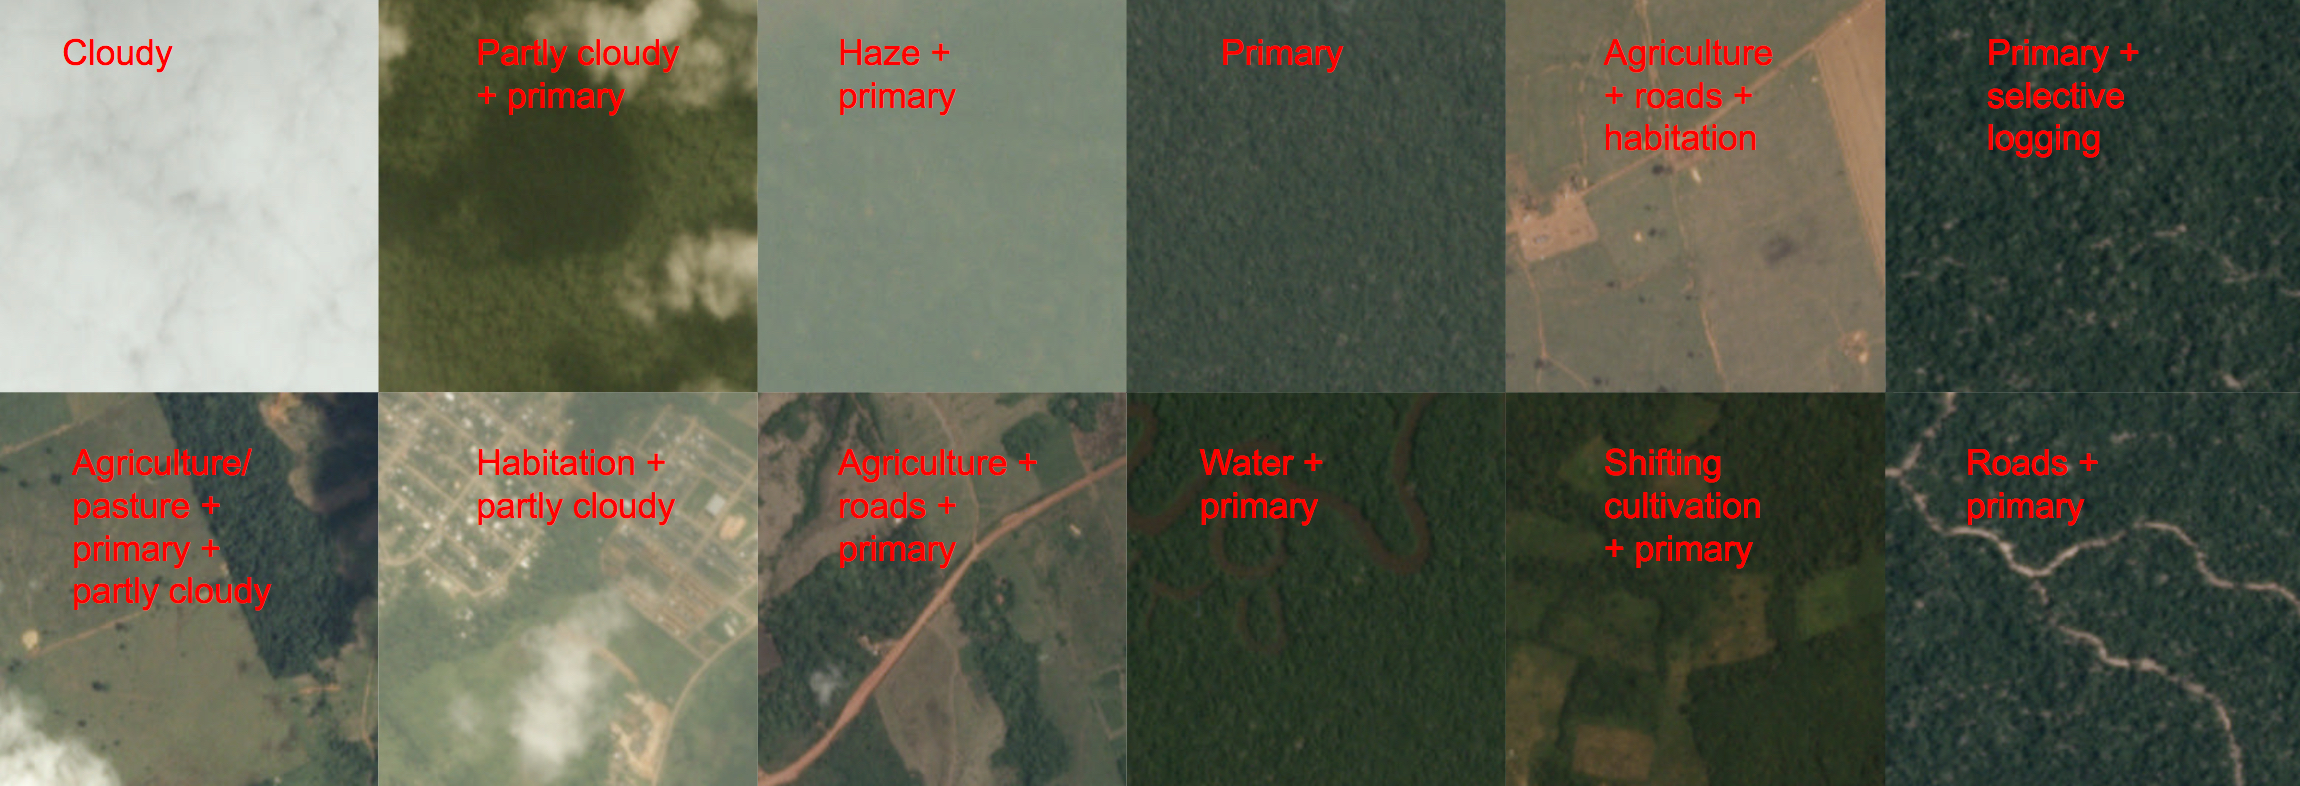
\includegraphics[width=0.75\linewidth, height=0.3\linewidth]{chips.jpg}
 \captionof{figure}{Sample chips and their labels.}\label{fig:sample}
\end{Figure}

\section{Datasets and Input}
\label{S:3}
Data\cite{amazonkaggle} are composed of 40479 labeled training images and 61191 unlabeled images for final submission. The file size of an original image is ${256\times 256 \times 3}$, I resize it to $128\times 128\times 3$.  The labeled data is splitted into $80\%$ training set and $20\%$ testing set. Fig~\ref{fig:labels} and Tab.~\ref{tab:labels} show the label distributions of the training and testing data.

\begin{multicols}{2}
\begin{Figure}
 \centering
 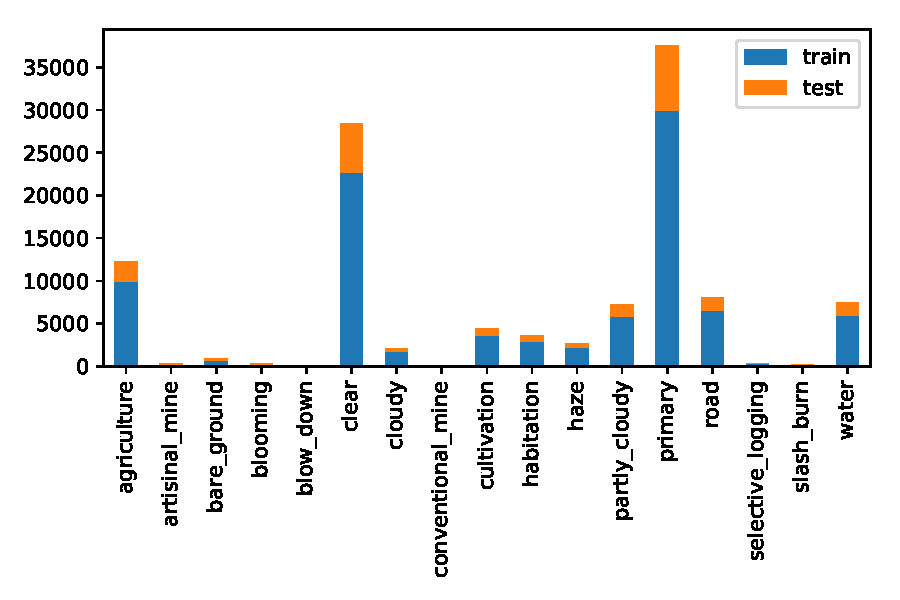
\includegraphics[width=\linewidth, height=1.\linewidth]{labels.pdf}
 \captionof{figure}{Labels distribution between training and testing}\label{fig:labels}
\end{Figure}
\small{
\begin{Figure}
\begin{tabularx}{1\columnwidth}{l|l|l|l}
\hline
\hline
Label & total & train & test \\ \hline
cloudy & 2089 & 1686 & 403\\ 
partly cloudy &  7261 & 5844 & 1417\\  
haze &   2697  & 2177 & 520 \\
clear &   28431 & 22676 & 5755 \\
primary & 37513 & 29977 & 7536\\
water & 7411  & 5941 & 1470 \\
habitation & 3660  & 2927 & 733 \\
agriculture & 12315 & 9950 & 2365\\
road & 8071 & 6490 & 1581 \\
cultivation & 4477 & 3560 & 917\\
bare ground & 862 & 698 & 164\\
slash burn & 209 & 171 & 38\\
selective logging & 340 & 285 & 55 \\
blooming & 332 & 260 & 72\\
conventional mine & 100 & 81 & 19\\
artisinal mine & 339 & 268 & 71 \\
blow down & 98 & 75 & 23\\ \hline
\end{tabularx}
\captionof{table}{Label classification of training/testing data.}\label{tab:labels}
\end{Figure}
}

\end{multicols}

%\begin{figure}[h]
%\centering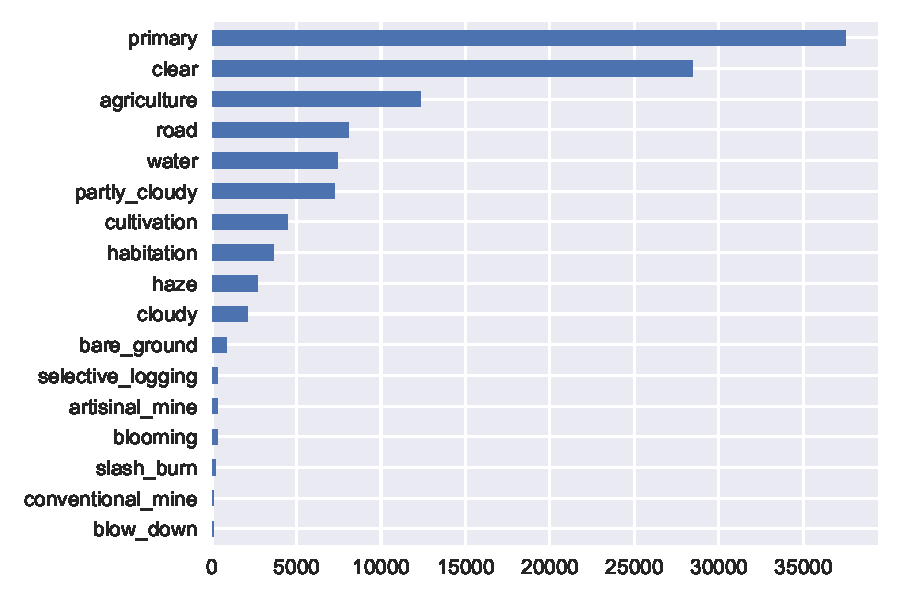
\includegraphics[width=0.6\linewidth]{amazon_labels.pdf}
%\caption{Label frequencies of training data.}
%\end{figure}  

%blow_down               98
%conventional_mine      100
%slash_burn             209
%blooming               332
%artisinal_mine         339
%selective_logging      340
%bare_ground            862
%cloudy                2089
%haze                  2697
%habitation            3660
%cultivation           4477
%partly_cloudy         7261
%water                 7411
%road                  8071
%agriculture          12315
%clear                28431
%primary              37513
  
\section{Solution and Statement}
\label{S:4}
There are two main methods to solve multi-label classification problem. One is to transform the multi-label problem into single label problems(s), but the transformed dataset grows large with high label cardinality and cannot model dependencies between labels. The other one is to adapt a single-label algorithm to produce multi-label outputs. In this competition, I will adapt conventional neural network with multiple outputs.

\subsection{Loss Function}
In single label classification, we use softmax function to squash the values of a vector in the range $[0,1]$ that add up to 1. In multi-label case, a sigmoid function Eq.~\ref{eq:sigmoid} is used to predict the outputs, which indicates the class probabilities. 
\begin{equation}
\sigma(x) = \frac{1}{1 + \exp{(-x)}} \label{eq:sigmoid}
\end{equation}

Binary cross entropy function is used as loss function Eq.~\ref{eq:loss},
\begin{eqnarray}
\mathcal{L}(\theta) & = &  
-\frac{1}{n}\sum^{n}_{i=1}\left[y_i \log(p_i) + (1-y_i)\log(1-p_i)\right] \nonumber \\
& = & -\frac{1}{n}\sum^{n}_{i=1}\sum^{m}_{j=1}y_{ij}\log(p_{ij}) \label{eq:loss}
\end{eqnarray}
where $i$ sums over all samples and $j$ sums over all classes, $y$ is the sample label and $p_{ij}\in(0,1)$,$\sum_{j} p_{ij} = 1 \forall i, j$ is the prediction for a sample.

\subsection{Measurement Metrics}
Evaluation of multi-label algorithm is hard mostly because of partial correctness of a prediction. One trivial way around is to ignore partially correctness and extend the accuracy used in single label case for multi-label prediction, see Eq.~\ref{eq:accuracy}
\begin{equation}
\mathrm{accuracy} = \frac{1}{N}\sum^{N}_{i = 1}\mathcal{I}(y^i = y^i_{\mathrm{pred}})\label{eq:accuracy}
\end{equation}

In this kaggle competition, the $F_2$ score is used to evaluate the submission, see Eq.\ref{eq:f2}
\begin{equation}
F_{2} = (1+\beta^{2})\frac{pr}{\beta^2 p + r}, \quad \beta = 2 \label{eq:f2}
\end{equation}
where Precision $p$ is the ratio of true positives to all predicted positives. Recall $r$ is the ratio of true positives to all actual positives. $F_2$ weights recall higher than precision, the mean $F_2$ score is formed by averaging the individual $F_2$ scores for each row in the test data. 

\subsection{Baseline Model}
Convolutional neural network (CNN) has demonstrated excellent performance on many complex visual tasks. CNN architecture has three major components:
\begin{itemize}
\item  Convolution layer: we slide the filters (weight matrices) over the complete image, and minimize the loss function to learn the weights. The filters contain features extracted from the original image, for example, one filter might learn edge and another one learn shape \emph{etc.} In general, the initial layer extract more generic features, when network goes deeper, the filters will learn more complex features. 
\item Pooling or Sub Sampling: we reduces the dimensionality of weight matrices but retains the most important information. There are different spatial pooling types: max, average, sum \emph{etc}.
\item Fully Connected Layer is a multi layer perceptron that uses a softmax activation function in the output layer for classification.
\end{itemize}

My baseline model is a two layers of CNN with three fully connected  layers. Each fully connected layer is followed by a pooling layers with drop probability $0.3$. Early stopping is used as regularization to avoid overfitting. Fig.~\ref{fig:cnngraph} shows the architecture of baseline CNN. Data is trained in $31$ epochs with batch size of $128$. Fig.~\ref{fig:baseline_metrics} shows accuracy, loss and $F_2$ score over $31$ training epochs, where the tagging threshold of prediction is $0.5$. However, multi-label is different from single label classification, in single label classification, we select label with highest score as prediction. In multi-label classification, the threshold for each label might be different, thus, I tune the label threshold to optimize $F_2$ of each label over the training data. For each label, I calculate $F_2$ scores using $20$ different thresholds that evenly spaced in range $[0.01, 0.99]$, then pick the one which maximizes the $F_2$ score.

\begin{multicols}{2}
\begin{Figure}
 \centering
 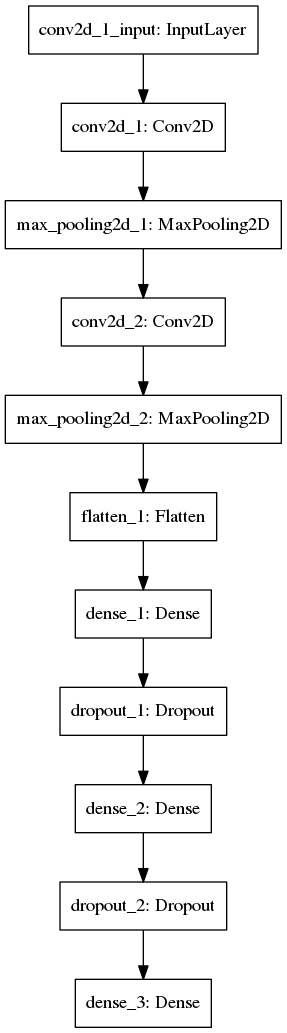
\includegraphics[width=0.4\linewidth, height=0.9\linewidth]{baseline_model.png}
 \captionof{figure}{Tensorboard: baseline CNN architecture.}\label{fig:cnngraph}
\end{Figure}
\begin{Figure}
 \centering
 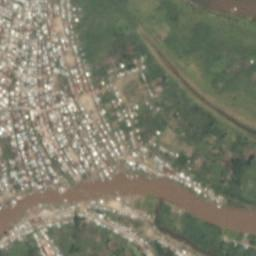
\includegraphics[width=0.7\linewidth]{train_9252.jpg}
 \captionof{figure}{True Label: agriculture clear habitation primary road water. \newline Prediction: agriculture clear habitation primary road}\label{fig:train9252}
\end{Figure}
\end{multicols}

\begin{Figure}
 \centering
 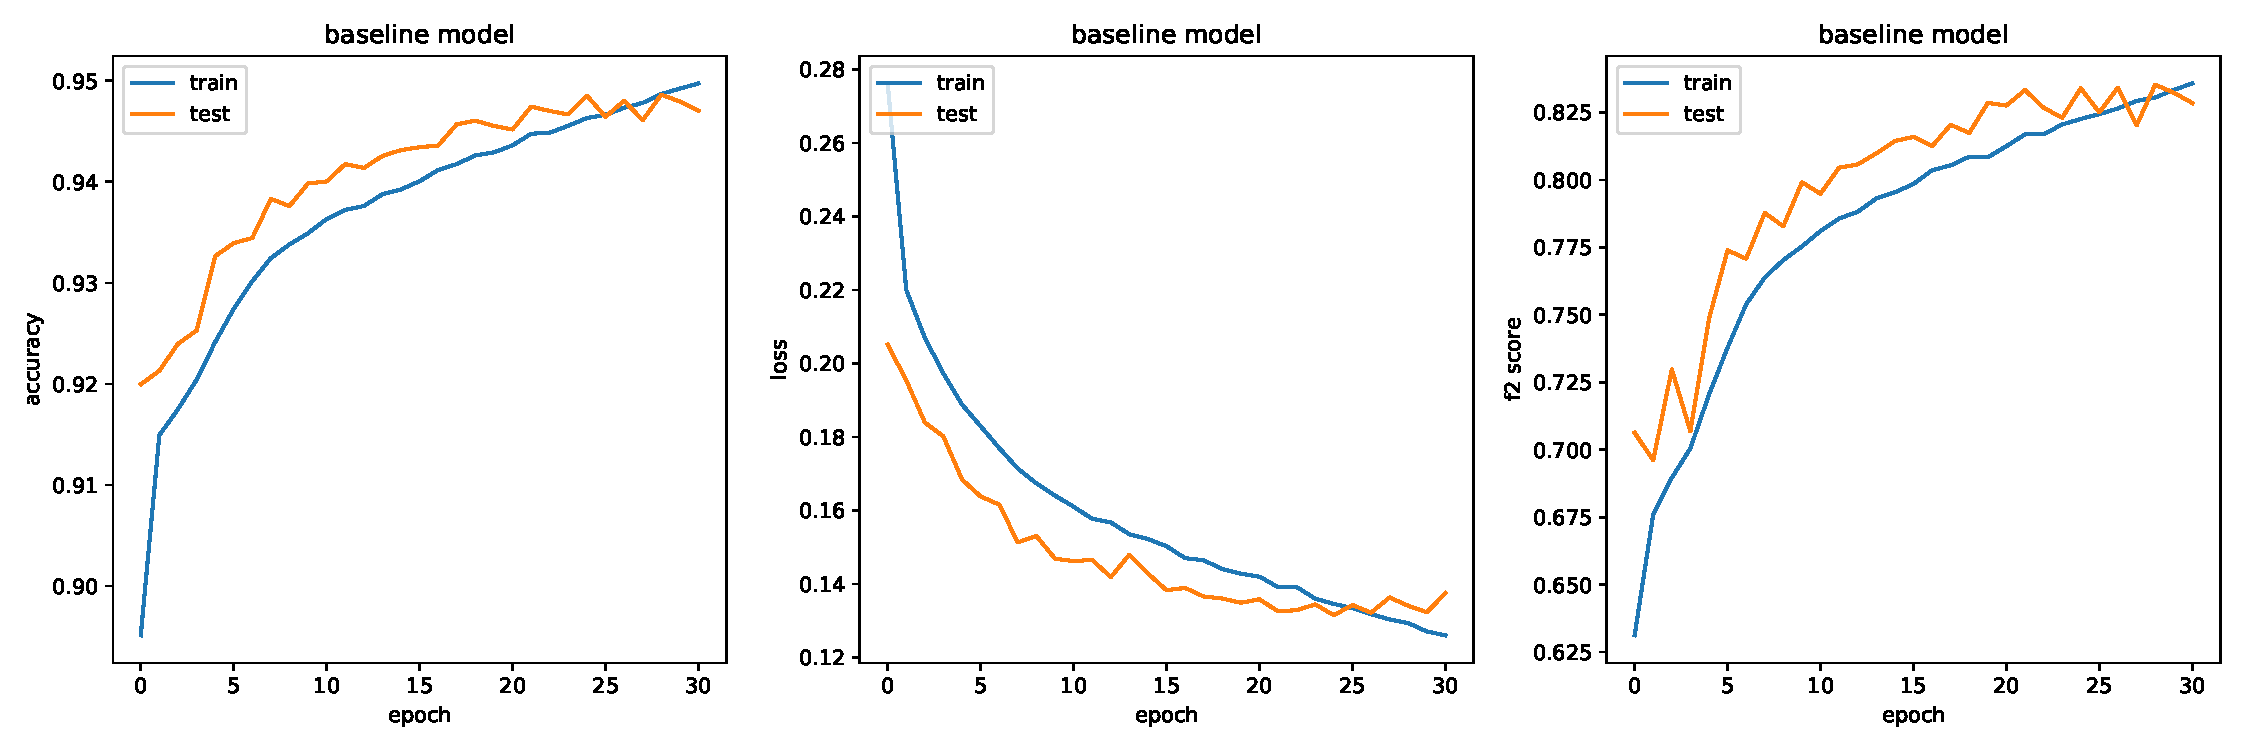
\includegraphics[width=1.\linewidth, height=0.33\linewidth]{baseline_metrics.pdf}
 \captionof{figure}{Accuracy, loss and $F_2$ score in each epoch}\label{fig:baseline_metrics}
\end{Figure}

Tab.~\ref{tab:baseline_f2} compares $F_2$ from using fixed threshold $0.5$ with those from using optimized threshold, which are improved especially for rare features. I submit the predictions using baseline model, $F_2$ score is $0.82752$ and $0.87329$ for using fixed threshold and optimized threshold respectively. (Tab.~\ref{tab:conclusion} lists the $F_2$ of training/testing data), sample submission benchmark from Kaggle is $0.67485$. 

\begin{table}[ht]
\begin{tabular}{l|c|c|c|c|c|c}
\hline
\hline
Label      & threshold & training $F_2$ & testing $F_2$ & threshold & training $F_2$ & testing $F_2$ \\\hline
cloudy            & 0.5  & 0.8396 & 0.7991 & 0.2679  & 0.8725 & 0.8184 \\ 
partly cloudy     & 0.5  & 0.9195 & 0.8347 & 0.2679  & 0.9406 & 0.8626 \\  
haze              & 0.5  & 0.5515 & 0.5428 & 0.1647  & 0.7614 & 0.7124 \\
clear             & 0.5  & 0.9724 & 0.9556 & 0.2163  & 0.9801 & 0.9714 \\
primary           & 0.5  & 0.9826 & 0.9831 & 0.2679  & 0.9886 & 0.9883 \\
water             & 0.5  & 0.3104 & 0.2636 & 0.1647  & 0.6741 & 0.6577 \\
habitation        & 0.5  & 0.4006 & 0.3403 & 0.1647  & 0.7038 & 0.6499 \\
agriculture       & 0.5  & 0.8062 & 0.7661 & 0.2163  & 0.8708 & 0.8346 \\
road              & 0.5  & 0.6362 & 0.6158 & 0.2163  & 0.8104 & 0.7823 \\
cultivation       & 0.5  & 0.1559 & 0.1097 & 0.1647  & 0.6312 & 0.6056 \\
bare ground       & 0.5  & 0.0    & 0.0    & 0.0616  & 0.3804 & 0.2814 \\
slash burn        & 0.5  & 0.0    & 0.0    & 0.0616  & 0.2018 & 0.0375 \\
selective logging & 0.5  & 0.0    & 0.0    & 0.0616  & 0.4332 & 0.1975 \\
blooming          & 0.5  & 0.0    & 0.0    & 0.0616  & 0.3157 & 0.2193 \\
conventional mine & 0.5  & 0.0    & 0.0    & 0.0616  & 0.1933 & 0.1773 \\
artisinal mine    & 0.5  & 0.2096 & 0.0865 & 0.2163  & 0.7410 & 0.4225 \\
blow down         & 0.5  & 0.0    & 0.0    & 0.0100  & 0.1123 & 0.0812 \\ \hline
\end{tabular}
\caption{Baseline model: label tagging threshold, and label $F_2$ score of training/testing}\label{tab:baseline_f2}
\end{table}


\subsection{Transfer Learning}
Transfer learning involves taking a pre-trained neural network and adapting the neural network to a new different data set and thus accelerate our deep learning model. There are two major methods in transfer learning: retraining and fine tuning, depending on the size of new data set and the similarity of new data to the original data. There are four main cases, see Tab.~\ref{tab:transfer}.
\begin{table}[ht]
\begin{tabular}{l|c|c}
\hline
\hline
& size of new data & similarity to original data \\\hline
case 1 & small & similar \\
case 2 & small & different \\
case 3 & large & similar \\
case 4 & large & different \\\hline
\end{tabular}
\caption{Transfer learning}\label{tab:transfer}
\end{table}

In transfer learning, we replace the last fully connected layer with a layer matching the number of classes in the new data set. 
\begin{itemize}
\item case 1: Freeze all the weights from the pre-trained network except the last layer, train the network to update the weights of the new fully connected layer.
\item case 2 : Remove most of the pre-trained layers near the beginning of the network, retrain the weights of final layer like case 1
\item case 3 : Fine tune the network by initializing weights except the last layer with the pre-trained weights and retrain the entire neural network.
\item case 4: Retrain the network from scratch with randomly initialized weights or try fine tuning.
\end{itemize}

\subsubsection{Inception v3 Architecture}
GoogleNet won the ILSVRC 2014 challenge by pushing the top-5 error rate below $7\%$. The great performance is achieved by a sub-network called Inception. Inception architecture, see Fig~\ref{fig:inceptionv3_arch}, stacks multiple Inception modules to a deep depth, and each module is also "wide" and architected to recognize features at multiple length scales. It includes $3\times3$ and $5\times5$ convolutions in each stacked module, as shown in Fig~\ref{fig:inception_naive}. However, these convolutions are expensive, and it is getting worse when repeatedly stacked them in a deep depth. To reduce dimensionality, a $1\times1$ convolution is stacked in front of the expensive $3\times3$ and $5\times5$ convolutions respectively, see Fig.~\ref{fig:inception_arch}.

\begin{Figure}
 \centering
 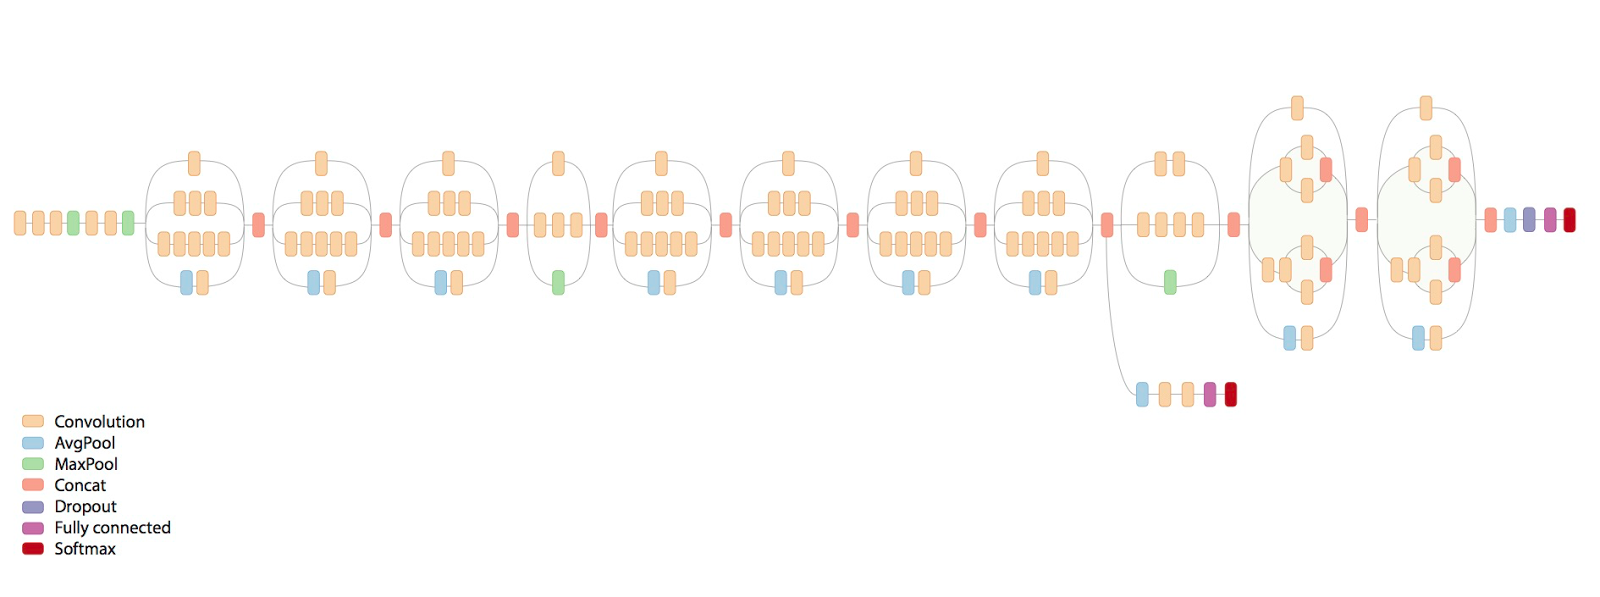
\includegraphics[width=1.\linewidth, height=0.26\linewidth]{inceptionv3_arch.png}
 \captionof{figure}{Inception v3 Architecture.}\label{fig:inceptionv3_arch}
\end{Figure}

\begin{multicols}{2}
\begin{Figure}.
 \centering
 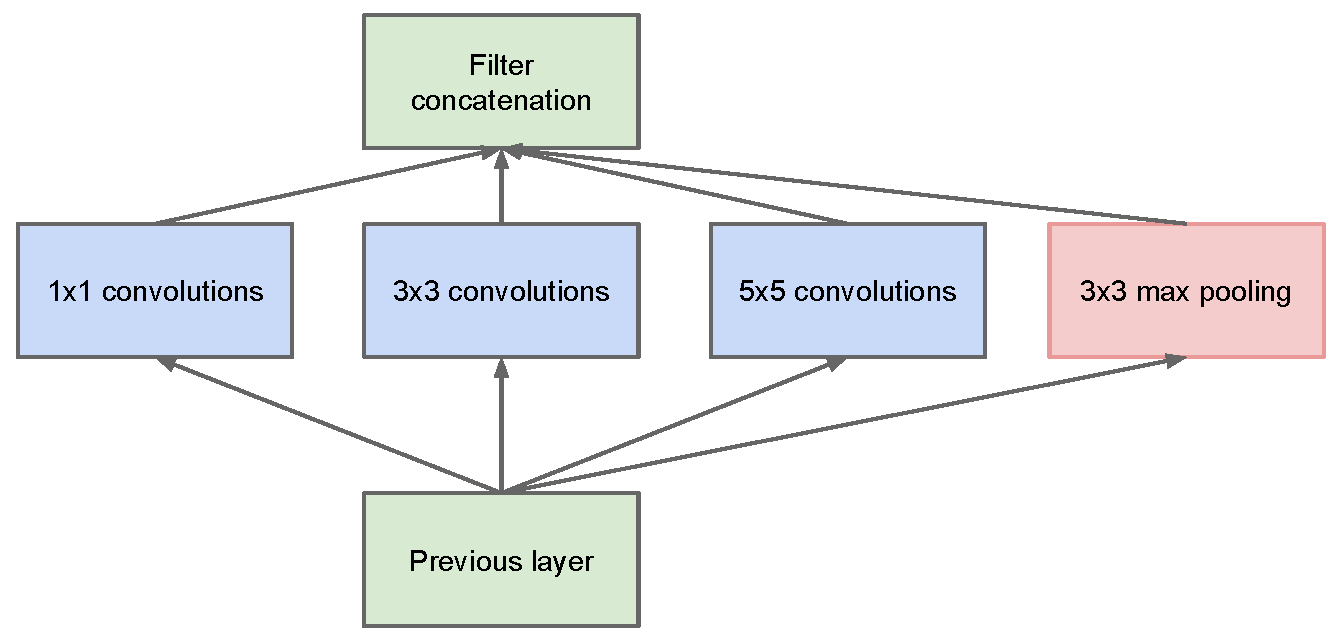
\includegraphics[width=\linewidth, height=0.5\linewidth]{inceptionnaive.pdf}
 \captionof{figure}{Naive inception module~\cite{goingdeeper}.}\label{fig:inception_naive}
\end{Figure}
\begin{Figure}
 \centering
 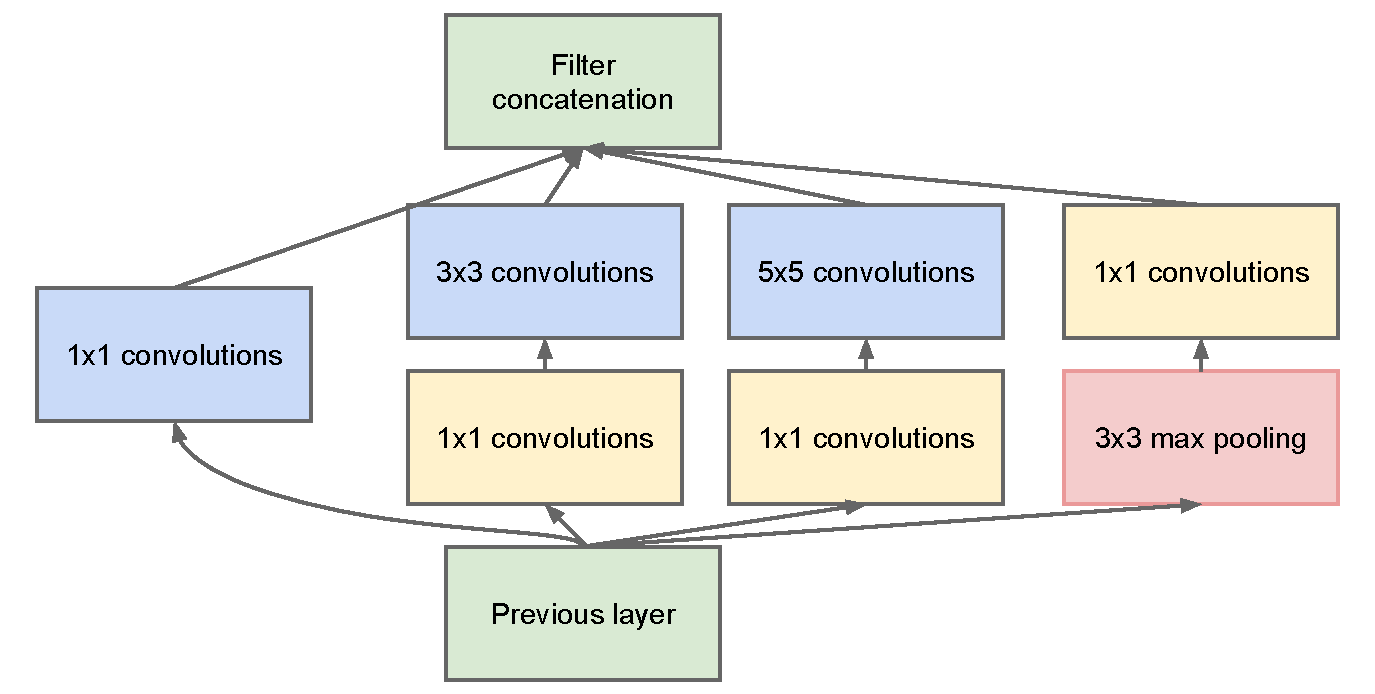
\includegraphics[width=\linewidth, height=0.5\linewidth]{inceptionmodule.pdf}
 \captionof{figure}{Inception module~\cite{goingdeeper}.}\label{fig:inception_arch}
\end{Figure}
\end{multicols}

\subsubsection{Retraining And Fine Tuning}
The amazon satellite image data set is medium, however, is different from ImageNet which used to train InceptionV3, VGG16 \emph{etc}. I load InceptionV3 model from keras, pop up the final layers and use a fully-connected layer in shape of $1\times1\times17$ as the final layer, where $17$ is the total number of classes of amazon images. ImageDataGenerator of keras is used to generate batches of augmented tensor image in realtime training, the images are randomly rotated, and horizontally/vertically shifted. Fig.~\ref{fig:train_augment} shows the augmentation strategy applied on original image in Fig.~\ref{fig:train9252}. Adam optimizer\cite{adam} is chosen to minimize the loss function Eq.\ref{eq:loss} with a constant learning rate of $0.0005$.

\begin{figure}[htbp]
    \hspace{-4mm}
    \begin{minipage}{0.33\linewidth}
        \centering
        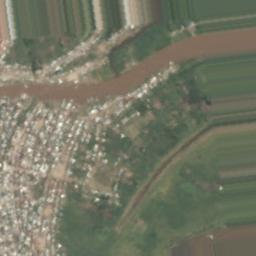
\includegraphics[width=1.4in]{train_9252_0_175.jpg}\\
    \end{minipage}
    \begin{minipage}{0.33\linewidth}
        \centering
        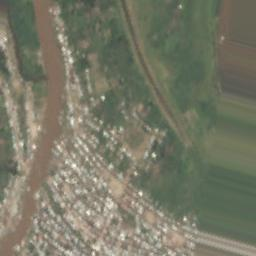
\includegraphics[width=1.4in]{train_9252_0_598.jpg}\\
    \end{minipage}
     \begin{minipage}{0.33\linewidth}
        \centering
        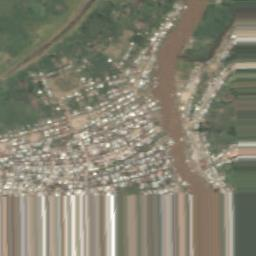
\includegraphics[width=1.4in]{train_9252_0_1710.jpg}\\
    \end{minipage}
    \caption{Augmented figures of Fig.~\ref{fig:train9252}.} 
    \label{fig:train_augment}
\end{figure}
\begin{Figure}
 \centering
 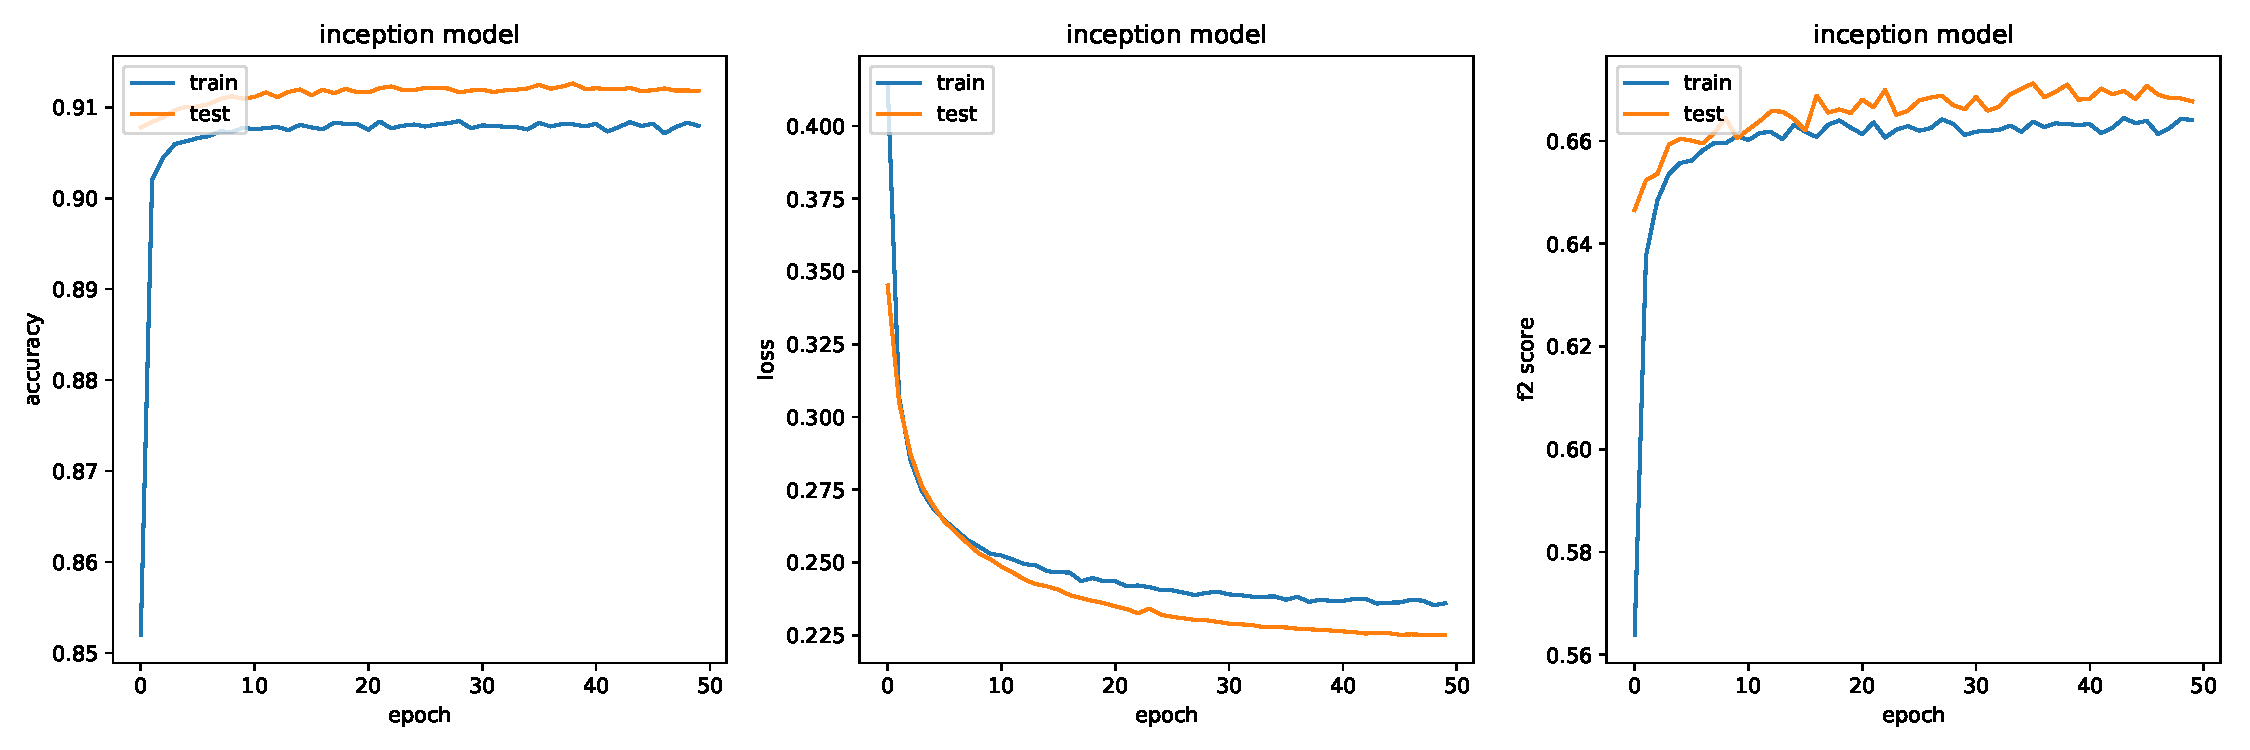
\includegraphics[width=1.\linewidth, height=0.33\linewidth]{inception_metrics.pdf}
 \captionof{figure}{Transfer learning: accuracy, loss and $F_2$ score in each epoch}\label{fig:inception_metrics}
\end{Figure}

I freeze all initial weights from training ImageNet except those in the last fully connected layer, retrain the network in $50$ epochs and save the checkpoint. Fig.~\ref{fig:inception_metrics} shows metrics in each epochs, all of which are worse than baseline model. Then I use the weights from retraining InceptionV3 as the initial weights and train the weights in all layers using $20$ epochs with a smaller learning rate of $0.0001$. In baseline model, optimized threshold gives a better prediction and higher $F_2$, therefore, I use the same method to find label thresholds.

Fig.~\ref{fig:inception_finetune_metrics} shows an improvement of accuracy, loss and $F_2$ score. Tab.~\ref{tab:inception_f2} shows the tagging threshold and $F_2$ of labels for training and testing data, from which $F_2$ score is improved for all labels and the improvement for rare features, like blow down, slash burn \emph{etc.} is noticable.

\begin{Figure}
 \centering
 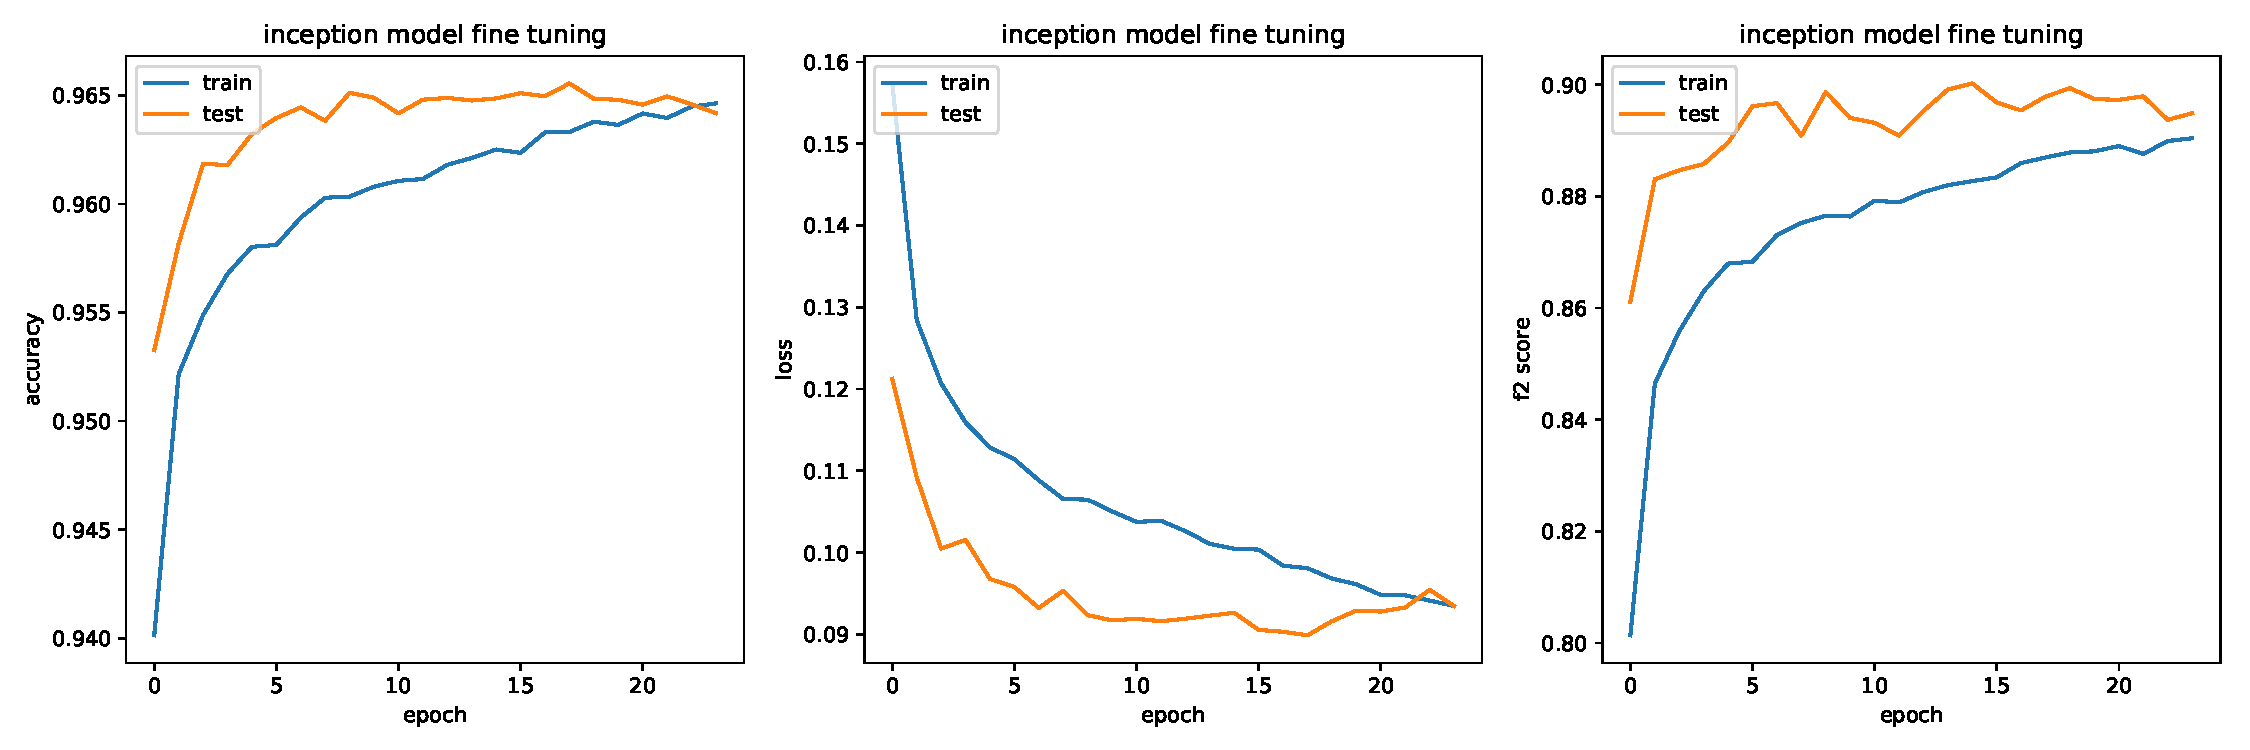
\includegraphics[width=1.\linewidth, height=0.33\linewidth]{inception_finetune_metrics.pdf}
 \captionof{figure}{Fine tuning InceptionV3: accuracy, loss and $F_2$ score in each epoch}\label{fig:inception_finetune_metrics}
\end{Figure}

%\small{
\begin{table}[ht]
\begin{tabular}{l|c|c|c}
\hline
\hline
Label & tagging threshold & training $F_2$ & testing $F_2$ \\\hline
cloudy             & 0.16474 & 0.9051 & 0.8832 \\ 
partly cloudy      & 0.21632 & 0.9520 & 0.9275 \\  
haze               & 0.16474 & 0.8115 & 0.7598 \\
clear              & 0.16474 & 0.9809 & 0.9731 \\
primary            & 0.31947 & 0.9910 & 0.9921 \\
water              & 0.16474 & 0.8271 & 0.8158 \\
habitation         & 0.16474 & 0.7671 & 0.7433 \\
agriculture        & 0.16474 & 0.9028 & 0.8936 \\
road               & 0.21632 & 0.8673 & 0.8489 \\
cultivation        & 0.16474 & 0.6957 & 0.6842 \\
bare ground        & 0.06158 & 0.5228 & 0.4480 \\
slash burn         & 0.06158 & 0.3113 & 0.3109 \\
selective logging  & 0.11316 & 0.5300 & 0.4218 \\
blooming           & 0.11316 & 0.4292 & 0.3167 \\
conventional mine  & 0.21632 & 0.7160 & 0.5376 \\
artisinal mine     & 0.21632 & 0.8656 & 0.8514 \\
blow down          & 0.11316 & 0.4669 & 0.3901 \\ \hline
\end{tabular}
\caption{Fine tuning InceptionV3: label tagging threshold, and label $F_2$ score of training/testing}\label{tab:inception_f2}
\end{table}
%}

\begin{Figure}
 \centering
 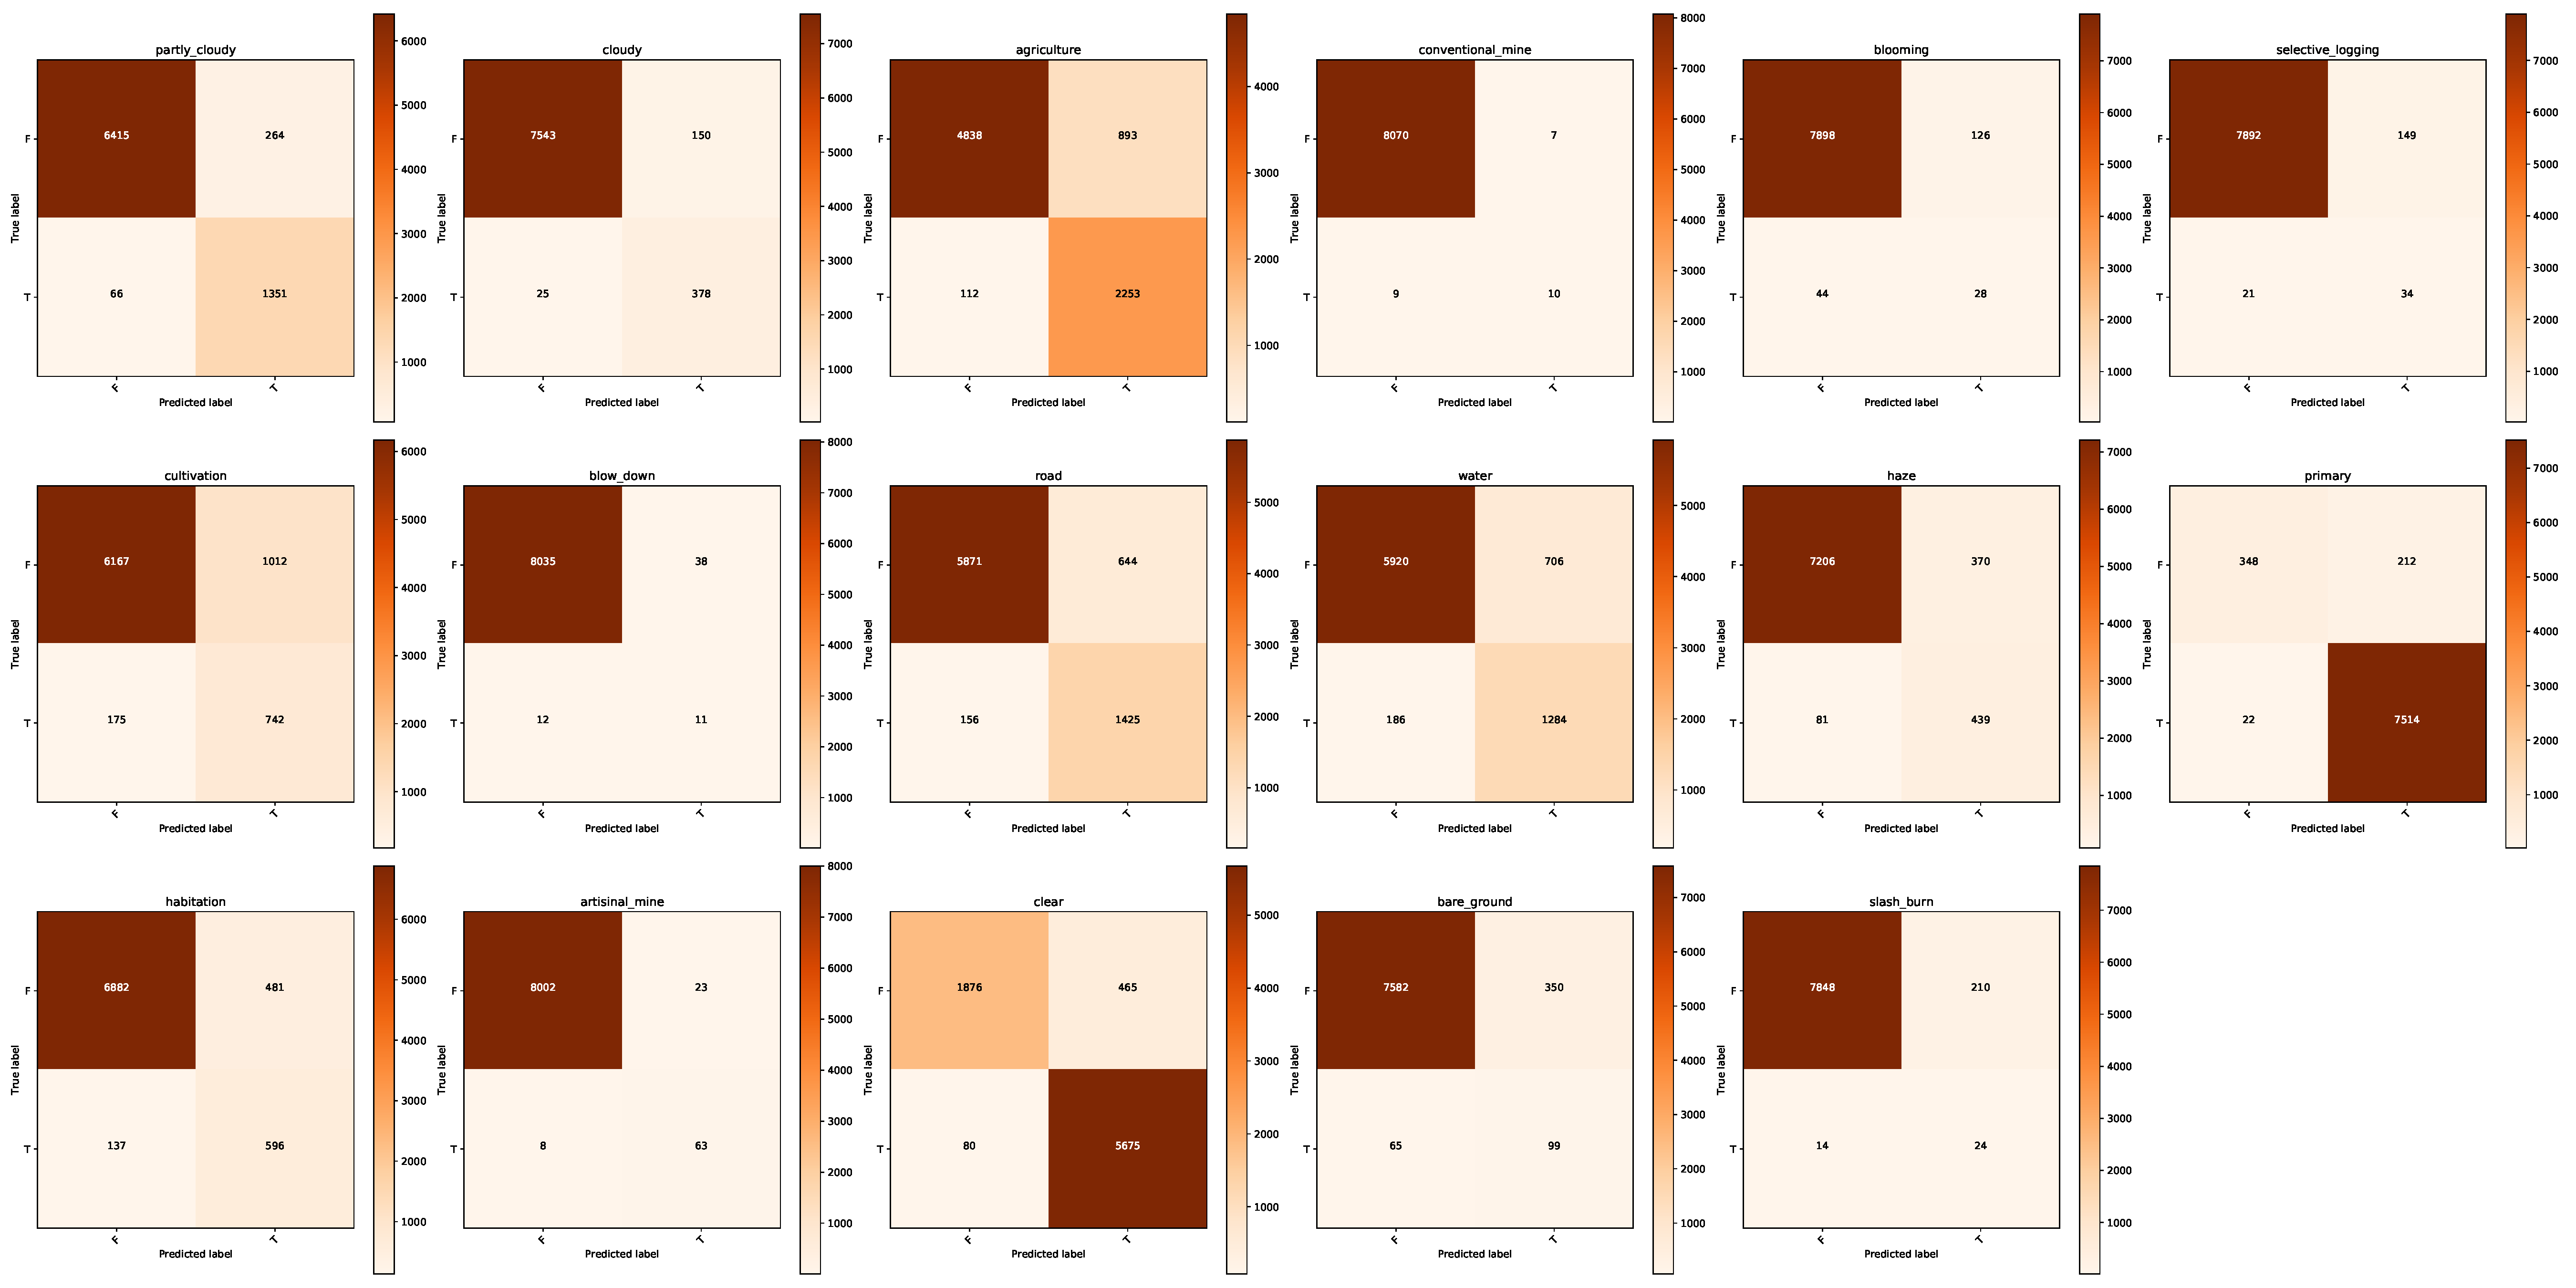
\includegraphics[width=1.1\linewidth]{label_cf.pdf}
 \captionof{figure}{Fine tuning InceptionV3: confusion matrices of labels calculated with testing data.}\label{fig:label_cf}
\end{Figure}

\subsection{Conclusion}
Tab.~\ref{tab:conclusion} shows the $F_2$ scores of training/testing data and final submission of unlabeled data using baseline model and fine tuning InceptionV3. $F_2$ score is improved by $\sim5\%$ when using transfer learning on InceptionV3. However it is still behind the highest $F_2$ score $0.93318$ in Kaggle lead board. Fig.~\ref{fig:label_cf} shows label confusion matrices calculated using testing data. For rare features, like 'bare ground', 'blooming' and 'selective logging', false negative is relatively large, indicating that my model is more likely to predicate false for rate features.

\begin{table}[ht]
\begin{tabular}{l|c|c|c}
\hline
\hline
                          &  $F_2$ training & $F_2$ testing & $F_2$ final submission \\
 \hline
Baseline (fixed threshold 0.5)           &  0.852129       &  0.834331  & 0.82752 \\
Baseline (optimized thresholds)          &  0.894239       & 0.874115      & 0.87329 \\
Fine tuning InceptionV3   &  0.928658       & 0.920617      & 0.91796 \\\hline
\end{tabular}
\caption{$F_2$ scores of training/testing data and final submission of unlabeled data for baseline model and fine tuning InceptionV3 model.}\label{tab:conclusion}
\end{table}

There are several ways to improve this multi-label learning. 
\begin{itemize}
\item Label distribution is unbalanced, $F_2$ and accuracy of rare features might be improved by generating more augmented images with rare labels.
\item Apply transfer learning on other pre-trained models like ResNet, VGG16, VGG19 \emph{etc.}, and compare the results with InceptionV3.
\item Apply ensembing method, which depends on  the  predictive  power of several models to make final prediction. 
\end{itemize}

%One method is to apply transfer learning on other pre-trained models like ResNet, VGG16, VGG19 \emph{etc.}, and compared the results with InceptionV3. Another potential method is ensembing, which depends on  the  predictive  power of several models to make final prediction. 

%% appendix sections are then done as normal sections
%% \appendix
%% \section{}
%% \label{}

%% References
%%
%% Following citation commands can be used in the body text:
%% Usage of \cite is as follows:
%%   \cite{key}          ==>>  [#]
%%   \cite[chap. 2]{key} ==>>  [#, chap. 2]
%%   \citet{key}         ==>>  Author [#]
%\end{multicols}
%% References with bibTeX database:
%\bibliography{mybib}{}
\bibliographystyle{unsrt}{}
\bibliography{citation}

%% Authors are advised to submit their bibtex database files. They are
%% requested to list a bibtex style file in the manuscript if they do
%% not want to use model1-num-names.bst.

%% References without bibTeX database:

% \begin{thebibliography}{00}

%% \bibitem must have the following form:
%%   \bibitem{key}...
%%

% \bibitem{}

% \end{thebibliography}
\end{document}

%%
%% End of file `elsarticle-template-1-num.tex'.